\section{Arduinoen og programmering} \label{sec:arduino}
\subsection{Arduino som komponent}
%--------------- Indsæt en arduino ---------------%
\begin{figure}[H]
	\centering
    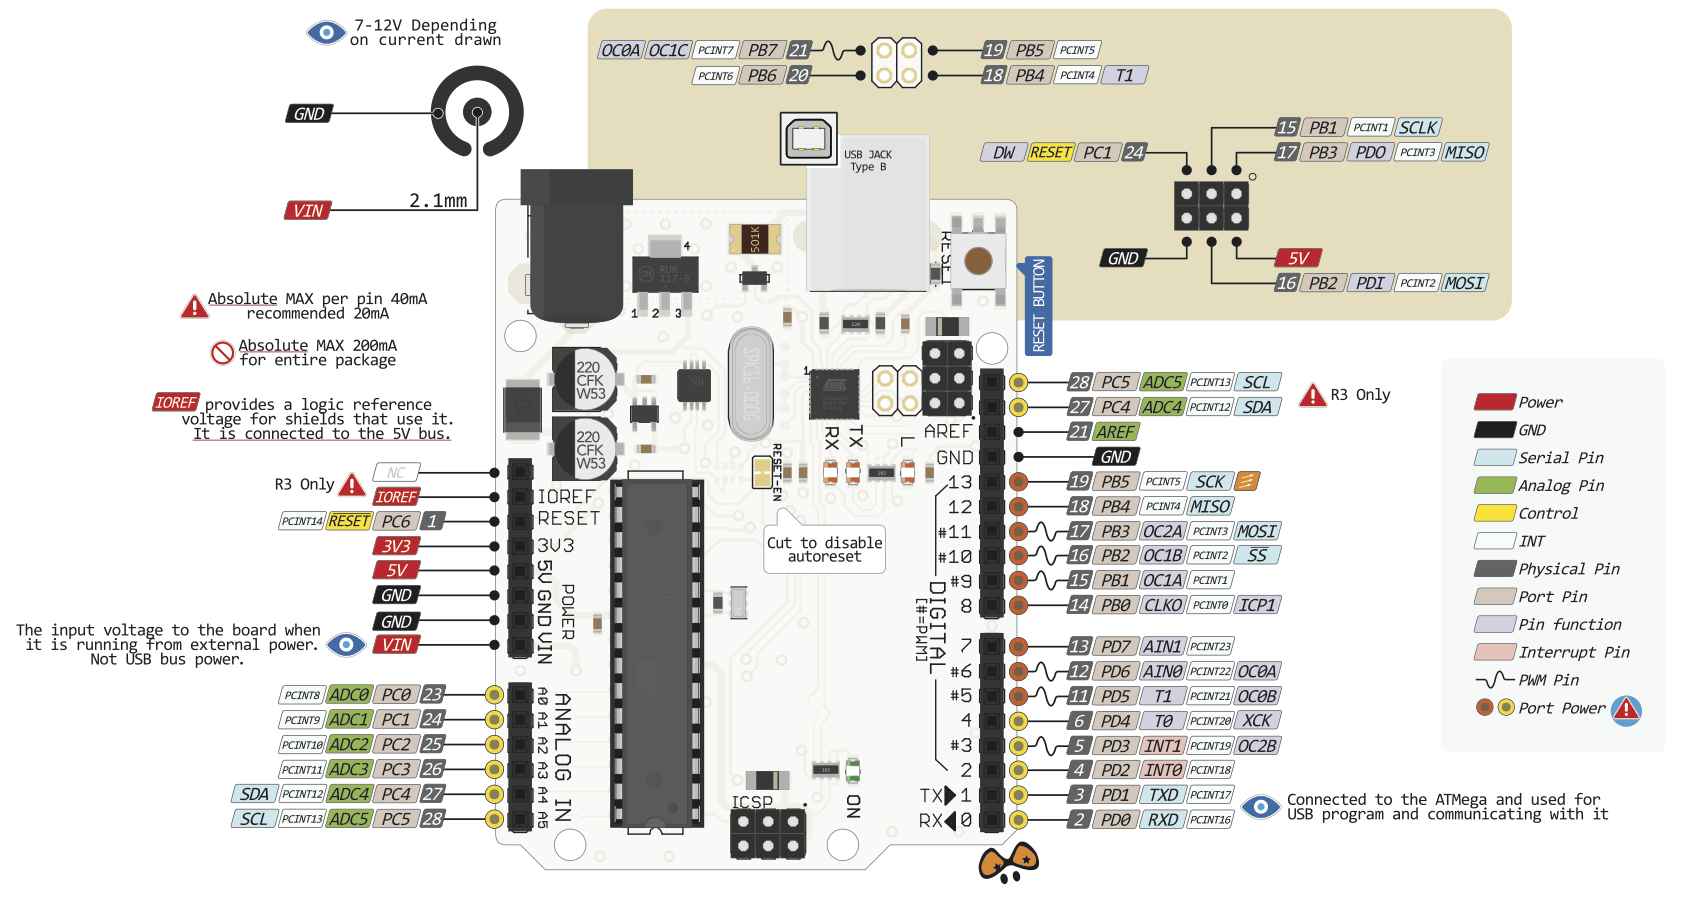
\includegraphics[width=\textwidth]{figures/arduino/portmani.PNG}
	\caption{Arduino uno med ATmega328}
	\label{fig:portmani}
	Her kan man se hvilke ben der er på Arduinoen, og hvilke porte de fordelt på ( PORTB, PORTC og PORTD). Hvis man ser på "Port pin", står der P for port, efterfulgt af bogstavet for hvilken port den er tildelt, efterfulgt af dens bit position i den port.\\
	Vi har også opgivet den påkrævede spænding for at køre Arduinoen. Vi kan også se Analog input ben (A0-A5) og de digital input og output ben (0-13). Vi kan se ud fra analog ben A4 og A5 at de er SDA og SCL, som er relevant når vi skal benytte I2C kredsen.
	\\Kilde: \url{http://pighixxx.com/unov3pdf.pdf}
\end{figure}
\subsubsection{Analog inputs og outputs (PWM)}\label{sec:ard:analog}
Analog input i Arduinoen er et input som beskriver spændingsfaldet over inputtet og jord med et 10 bit tal.\cite{arduinoAnalog} Dette betyder at den laveste værdi og højeste værdi af et analog input er
\begin{align}
\SI{}{U_{MIN}}&=b00\,0000\,0000\rightarrow 0\rightarrow \SI{0}{V}\\
\SI{}{U_{MAX}}&=b11\,1111\,1111\rightarrow 1023\rightarrow \SI{5}{V}\\
\end{align}
Med Arduinoen kan man få et analog input igennem en analog ben (se \ref{fig:portmani}), og kalde metoden \emph{analogRead()} til benets nummer, eksempelvis A0. Da vores precision er på 10 bit, til at beskrive et maks spændingsfald på $\SI{5}{V}$, må det gælde at den laveste ændring i spændingsfaldet vi kan måle er
\begin{align}
U_{prec}&=\frac{\SI{5}{V}}{1023}\approx \SI{5d-3}{V}
\end{align}
\subsubsection{Digital inputs og outputs}
Digital input på Arduinoen er en boolean værdi, som enden kan være sand eller falsk (også kendt som TRUE/FALSE eller HIGH/LOW). Disse værdier reflektere den digitale logik på det digitale ben, som fungere således: når spændingsfaldet mellem bennet og jord er $\SI{5}{V}$ er værdien sand og når spændingsfaldet er $\SI{0}{V}$ er den falsk. Mere præcist skifter værdien mellem at være sand og falsk ved omkring $\SI{3}{V}$, på $\SI{5}{V}$ logik Arduinoer. \cite{arduino:dig}\\
\\
Et digital output følger samme logik, her der sætter man dog udgangsspændingen på bennet. Det betyder altså at hvis man sætter et digital ben til sandt, vil udgangsspændingen på bennet være $\SI{5}{V}$ og hvis man sætter det til falsk vil det være $\SI{0}{V}$. \cite{arduino:dig}\\
\\


\subsubsection{Portmanipulation og registrer}
I Arduinoen bliver der brugt 8 bit registrer til at styre Arduinoens ben. Et register en type hukommelse der ofte er sammensat af flip flops. En type register er et parallelt register, som har et ben for hvert bit, således at værdien af den bit kan sættes med det ben. Disse kan bruges til eksempelvis at bestemme retningen af et ben (input/output) eller huske tilstanden af digitale ben.\\
\\
I Arduinoen bliver der brugt 8 bit register, som betyder at der skal flere forskellige registre til at kortlægge alle benene på Arduinoen. Disse forskellige grupper af registre kalder man porte og på figuren \ref{fig:portmani}, kan man se hvilke ben der er på hvilke porte. Som man kan se på figuren, er der tale om tre forskellige porte, B, C og D. \\
\\
I hver port er der primært tale om tre forskellige register. DDR registret er registret hvor at benenes tilstand er gemt i. Det betyder for eksempel at når man kalder funktionen \textit{pinMode(pin,mode)} finder Arduinoen først ud af hvilket registre \textit{pin} høre til, og derefter finder dens plads i registret og derefter ændre tilstanden af den bit til \textit{mode}. Her har man simplificeret processen i at ændre tilstanden af et ben, men ofret hastighed.
\\
\\
De to andre primære registre er PORT og PIN. PORT registret indeholder værdien af benene (højt eller lavt), som man også kan ændre på, hvis benet er registreret som et output i DDR registret. PIN indeholder også værdien af benene, har har man dog kun mulighed for at læse på værdien, og ikke ændre værdien. Man ville sige at PIN har samme funktion som PORT, men er \textit{write protected}, således at man ikke ved et uheld ændre en værdi på et ben.
\\
\\
Man kan med fordel benytte registrer, hvis programmet skal køre hurtigere, eller en process kræver at flere bens værdi bliver læst samtidig. Et eksempel på dette er når vi gerne vil overføre knappernes tilstand fra Controlleren. Her kan vi benytte portmanipulation til at få værdien af flere ben som en enkelt byte, hvis man da har valgt ben som er på samme port. I vores tilfælde benytter vi A0, A1 og A2 til knapper, som heldigvis ligger på samme port. Dette betyder at vi kan læse alle benenes digitale værdier ved at læse PORT eller PIN til porten. I programmet for Controlleren er der en funktion \textit{requestEvent()}, som skal sende tilstanden af knapperne. Den ser således ud når portmanipulation bruges.
\begin{lstlisting}
void requestEvent() {
  //Antager at A2, A1 er høje og A0 er lav 
  byte data = PINC; //Port C input registret
  //data = b0000 0110
  Wire.write(data); //Sender dataen over I2C
}
\end{lstlisting}
Den ville se således ud hvis portmanipulation ikke bliver brugt.
\begin{lstlisting}
void requestEvent() {
  //Antager at A2, A1 er høje og A0 er lav 
  byte data =digitalRead(A2);
  //data = b0000 0001
  data=data<<1+digitalRead(A1);
  //data = b0000 0011
  data=data<<1+digitalRead(A0);
  //data = b0000 0110
  Wire.write(data); //Sender dataen over I2C
}
\end{lstlisting}
Har kan vi se at ved at benytte PINC registret fik vi både simplificeret processen, og gjort den hurtigere. Et kald til et registre som PINC tager omkring 1 instruktion som er meget hurtigere end at kalde \textit{digitalRead(pin)} 8 gange, eller i vores tilfælde 3 gange. Resten af programmet kan findes i bilag \ref{bilag:programController}.\\
\\
Kilde \cite{arduino:port}.
\subsubsection{I2C - Synkroniseret kommunikations bus}
I2C står for "Inter-Integrated Circuit" som er en type serial kommunikations bus. I2C tillader flere komponenter at kommunikere med hinanden, kun ved brug af en fælles data ledning (SDA) og clock ledning (SCL). Dette betyder at alle komponenter på en I2C bus har en addresse, ofte i form af en 7 bit eller 8 bit værdi. I en I2C bus omdeler man komponenterne i to grupper; slaver og master. Slaver har ikke tilladelse til at sende data på bussen, ved mindre den er blevet anmodet om det, mens master kan sende data ud uden at blive anmodet.
\\
\\
Hvis vi tager udgangspunkt i vores produkt, er Controlleren en slave og den anden en master. Når master anmoder om noget fra Controlleren, så som værdien af knapperne, sender den først et START signal som indikere til andre master på bussen at bussen er optaget, derefter sender den adressen af det komponent den anmoder data fra. Her skal slaven som bliver anmodet sende et "Acknowledge", som indikere at den er klar til at modtage. Her indikere master så hvor mange bytes den anmoder om, hvorefter slaven sender det antal bytes. Når master så har modtaget dette bliver der sendt et STOP til bussen, som betyder at bussen ikke er optaget længere.\\
\\
Det praktiske ved I2C bussen er at det kræver få ledninger, netværket er nemt at udvide og et komponent på bussen kan blive "interrupted" (afbrudt). Dette betyder at hvis slaven er i gang med nogle beregninger, kan den blive afbrudt, hvis masteren anmoder om data. Dette betyder at I2C er ideel i vores tilfælde, hvor at vi har brug for at Controlleren (slaven) svare hurtigt når master anmoder om knappernes tilstande, så brugeren ikke føler "forsinkelse" fra når man klikker på knapperne og kanonen rykker sig. Vi benytter biblioteket "Wire" til at håndtere I2C kommunikation.
\\
\\
Kilde \cite{arduino:ITWOC}
%-------------------------------------------------------------------------------------------------------------------------------------------
%--------------------------------------- PROGRAMMING PART ----------------------------------------------------------------------------------
%-------------------------------------------------------------------------------------------------------------------------------------------
\subsection{Kort beskrivelse af programmets formål}
\subsubsection{Master Arduino}
Vores Master Arduino står for styring af motorerne, ladningssensor og hastighedssensor. Programmet til Master Arduinoen skal kunne kommunikere med Controlleren, så den kan se om der skal rygges op eller ned på kanonen eller om der skal affyres. Den skal også kunne bestemme farven af bolden i røret og om der faktisk er en bold i røret. Når bolden bliver affyret skal hastigheden af bolden også kunne bestemmes. Til sidst skal den kunne sende information som farven af bolden, hældningen af kanonen og hastigheden af bolden til Controlleren, så det kan skrives på displayet.
\subsubsection{Controller Arduino}
Controller Arduinoen skal kunne sende data om knappernes tilstand og kunne modtage data om hvad der skal stå på displayet. Da vores bruger benytter Controlleren til at styre kanonen, skal forsinkelsen imellem at man trykker på en knap, til at kanonen ryger sig være relativ lille.\\
\\
\\
\\
Programmet til master Arduinoen kan fines i bilag \ref{bilag:programMaster} og Controller Arduinoen i bilag \ref{bilag:programController}, som er kommenteret. De mest komplekse og primære funktioner vi har programmeret, er beskrevet i sektion \ref{sec:primaerefunc}.
\subsection{Oversigt over inputs og outputs og lokation}
\begin{table}[H]
	\caption{Inputs og outputs for Master Arduinoen} % title
	\label{tab:IOMaster}
	\centering
		\begin{tabular}{c|c c} 
		Ben & I/O & Forbundet komponent\\ [0.5ex] 
		\hline 
			2 & Output & Stepper motor\\
			3 & Output & Stepper motor\\
			4 & Output & Stepper motor\\
			5 & Output & Stepper motor\\
			6 & Output & Trækmotor\\
			9 & Output & Gearmotor (fri)\\
			10 & Output & Gearmotor (lås)\\
			11 & Output & Ladningssensor LED (grøn)\\
			12 & Output & Ladningssensor LED (rød)\\
			13 & Output & Ladningssensor LED (blå)\\
			A0 & Input & Ladningssensor Fotodiode\\
			A1 & Input & Hastighedssensor 1\\			
			A2 & Input & Hastighedssensor 2\\
			A4 (SDA) & I/O & I2C kommunikation (data)\\
			A5 (SCL) & I/O & I2C kommunikation (clock)\\[1ex]
		\hline %inserts single line
	\end{tabular}
\end{table}

\begin{table}[H]
	\caption{Inputs og outputs for Controller Arduinoen} % title
	\label{tab:IOController}
	\centering
		\begin{tabular}{c|c c} 
		Ben & I/O & Forbundet komponent\\ [0.5ex] 
		\hline 
			2 & I/O & LCD (DB7)\\
			3 & I/O & LCD (DB6)\\
			4 &I/O & LCD (DB5)\\
			5 &I/O & LCD (DB4)\\
			11 & Output & LCD (E)\\
			12 &Output & LCD (RS)\\
			A0 & Input & Knap (ryg kanon op)\\
			A1 & Input & Knap (ryg kanon ned)\\			
			A2 & Input & Knap (affyre bold)\\
			A4 (SDA) & I/O & I2C kommunikation (data)\\
			A5 (SCL) & I/O & I2C kommunikation (clock)\\[1ex]
		\hline %inserts single line
	\end{tabular}
\end{table}
\subsection{Kort beskrivelse af funktioner}\label{sec:primaerefunc}
\subsubsection{Master Arduino - Loop()}
\begin{figure}[H]
	\centering
    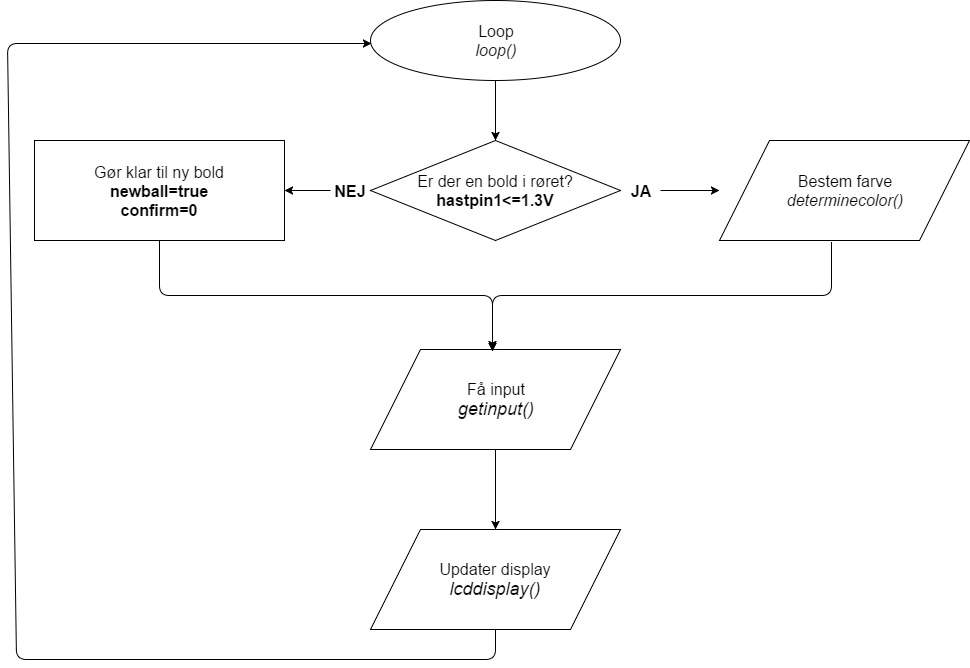
\includegraphics[width=\textwidth]{figures/arduino/M-loop.png}
	\caption{Flowchart af main loop hos Master Arduinoen}
	\label{flow:loop}
\end{figure}
Da vores første hastighedssensor er det sted i røret, hvor bolden vil hvile, ses der først om den første hastighedssensor er blokeret. Hvis den er blokeret, så kald funktionen \textit{determinecolor()}. Denne funktion bestemmer farven af bolden. Hvis hastighedssensoren ikke er blokeret, skal den nulstille nogle værdier, så den er klar til den næste bold.\\
\\
Efter alt dette skal funktionen \textit{getinput()} kaldes. Denne funktion får knap værdierne fra Controlleren, altså brugerinputtet. Derefter opdateres displayet med funktionen \textit{lcddisplay()}, som sender dataen som skal være på displayet over til Controlleren. Derefter starter \textit{loop()} forfra.

\subsubsection{Master Arduino - getinput()}
\begin{figure}[H]
	\centering
    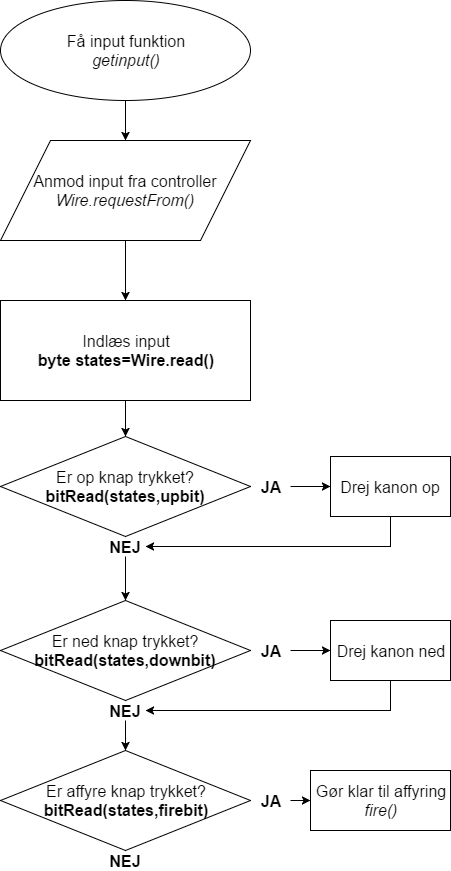
\includegraphics[height=15cm]{figures/arduino/M-getinput.PNG}
	\caption{Flowchart af input() funktionen hos Master Arduinoen}
	\label{flow:input}
\end{figure}
Det første der sker når \textit{getinput()} bliver kaldt, er at anmode om knappernes værdier fra Controlleren, med funktionen \textit{Wire.requestFrom()}. Derefter læses den byte som der sendes fra Controlleren. Denne byte indholder værdien af de 3 knapper. Her benyttes \textit{bitRead()} funktionen til at læse den bit på position upbit. Hvis denne bit er sand skal kanonen drejes op. Derefter tjekkes om nedbitten er sand. Hvis den er dette så skal kanonen drejes ned.
Derefter tjekkes om affyringsbitten er sand. Hvis den er dette skal funktionen \textit{fire()} kaldes, som affyre bolden, hvis der er en bold i røret.

\subsubsection{Master Arduino - fire()}
\begin{figure}[H]
	\centering
    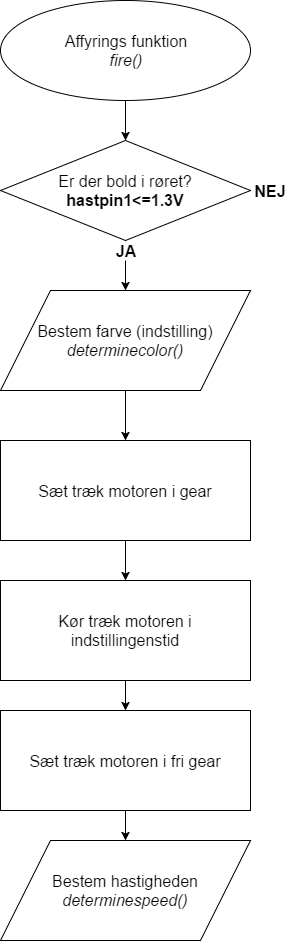
\includegraphics[height=15cm]{figures/arduino/M-fire.PNG}
	\caption{Flowchart af fire() funktionen hos Master Arduinoen}
	\label{flow:fire}
\end{figure}
Når \textit{fire()} funktionen bliver kaldt, ses der først om der er en bold i røret, ved at se om den første hastighedssensor er blokeret. Hvis den ikke er dette, så stop funktionen. Ellers fortsæt til at bestemme farven, som er indstillingen. Når farven er bestemt, sæt træk motoren i gear, således at elastikkerne kan trækkes i. Derefter kør træk motoren i den mængde tid som indstillingen siger. Derefter sæt træk motoren i frigear og stop træk motoren. Nu er elastikkerne i gang med at trække sig sammen igen. Her kaldes funktionen \textit{determinespeed()} til at bestemme hastigheden som bolden bliver skudt ud med.

\subsubsection{Master Arduino - determinespeed()}
I \textit{determinespeed()} beregner vi hastigheden af bolden. Dette gøres ved at se hvor lang tid det tager bolden at flyve afstanden imellem hastighedssensor 1 og 2. Hvis vi siger at afstanden imellem dem er $s$ og tiden det tager bolden at flyve denne afstand er $\delta T$, så kan hastigheden beregnes
\begin{align}
v=\frac{s}{\delta T}
\end{align}

\subsubsection{Master Arduino - determinecolor()}
\textit{determinecolor()} bestemmes farven. Vi arbejder med 4 forskellige farver; hvid, rød, grøn og blå. Da vores farvesensor ikke altid får den rigtige farve, bruger vi en værdi \textit{confirm} som angiver hvor mange gange farvesensoren har fået den samme farve. Hvis farvesensoren har fået den samme farve \textit{confirmAmount} gange i træk, så sættes \textit{newball} til falsk, som betyder at farven er bekræftet. Dette betyder dog også for affyringsfunktionen \textit{fire()}, at der kun kan affyres, når boldens farve er bekræftet. Dette kan i nogle tilfælde tage noget tid, hvis farvesensoren for den forkert et par gange.\\
Måden af \textit{determinecolor()} bestemmer farven, er ved først at lyse med en hvid farve på bolden. Hvis værdien fra farvesensoren er over en vis værdi, er farven hvid. Ellers bliver der lyst med rød, grøn og blå farve efter hinanden, hvor målinger bliver taget.